% ======================================================================
% CVPR 2026 Workshop: Foundation Models for Medical Vision
% Challenge: Foundation Models for General CT Image Diagnosis
% Task 1 (Linear Probing) -- All Data Track
% Team: maest   |   Method: MAE-ST (video-style spatiotemporal MAE for CT;
%                            forked from facebookresearch/mae_st)
% ----------------------------------------------------------------------
% NOTE TO AUTHORS: cells marked \tba{} need a final value or check before
% camera-ready. See NOTES_FOR_AUTHORS.md for the full list.
% ----------------------------------------------------------------------
% REVISION 2 -- addresses the three OpenReview reviews (ReNA, udzJ, 5vvC).
% Text-only; no number in the paper changed except where it was wrong.
%   Factual corrections
%     * visible-token counts: 627/157 -> 313/78  (models_mae.py: the encoder
%       sees int(784*(1-r)), so r=0.6 -> 313 and r=0.9 -> 78; the "4x more
%       context" ratio is unchanged, 313/78 = 4.0).           [ReNA]
%     * runtime rank: "second-fastest among the top four" -> third-fastest
%       (4.393, 4.467, 6.273, 9.414).                          [ReNA]
%     * Table 5 rank column typo: raidium was listed as rank 1, now 2.
%     * Fig. 2 caption: training ran to epoch 134, not 133 (last logged epoch
%       in the pre-training log is 134; last checkpoint written is 130).
%   Consistency
%     * the ablation difference count is now ELEVEN everywhere (abstract,
%       Sec. 2.1 "ten others", Sec. 3.4, Table 4, limitations, conclusion),
%       verified against the args saved in the v1 checkpoint (job 15124346,
%       checkpoint-00099.pth) and the v2 run (job 15326473). [ReNA, 5vvC]
%     * epoch-40 mean AUROC filled in: 0.646 (eval_v2_ep40_15327806.log).
%     * Table 4 difference list replaced -- see the comment above that table.
%   Claims softened to match the evidence                      [ReNA, udzJ, 5vvC]
%     * abstract / contribution 1 / Sec. 2.1 / conclusion no longer present
%       dynamic masking or the coarse temporal patch as demonstrated drivers.
%   New material answering reviewer questions
%     * Sec. 3.1 "Train/validation split": the split is organizer-provided
%       (the `split` column of the released per-target label CSVs); val is
%       exactly 50% positive for all 15 targets, train is 6.4-50%.    [udzJ Q2]
%     * Sec. 2.2: tail window is anchored at [D-16, D), never padded; edge
%       replication only when D < 16; ROI range re-centred if < 16 slices.
%                                                                     [udzJ Q1]
%     * Sec. 3.2 (3)+(4): stopping criterion (no validation signal; manual stop
%       on the loss plateau after epoch 134; schedule truncated, not annealed)
%       and why epochs 40 and 130 were the candidates.                [udzJ Q4]
%     * Sec. 2.2 "Linear-probe head" + Table 3 caption: C and checkpoint were
%       both selected on the reported split -> values are selection-optimistic
%       upper bounds; BalAcc threshold is 0.5 and equals accuracy on a balanced
%       split.                                                        [5vvC W2]
%     * Sec. 3.6 states the aggregation rule as an explicit assumption, notes
%       that the organizers do not publish it (their eval code computes
%       per-target metrics and never aggregates; the scoring program is not
%       released), and shows the decomposition is insensitive to it: macro mean
%       -> chest would need 0.219 / shortfall 0.037; sample-weighted -> 0.290 /
%       0.034. Either way chest cannot absorb the gap.            [5vvC W1(a)]
%     * NEW Sec. 3.6 + Table 6: quantitative decomposition of the 0.678 -> 0.624
%       difference. Chest-at-chance explains only 0.021 of the 0.054; the
%       implied abdominal test mean is ~0.641. Replaces the old claim that the
%       two chest targets explain the whole gap.                      [5vvC W1]
%     * Limitations restructured into Evaluation / Attribution / Generalization,
%       naming the exact follow-up runs that would settle each point.
% ======================================================================
\documentclass[runningheads]{llncs}

\usepackage[T1]{fontenc}
\usepackage{multirow}
\usepackage{graphicx}
\usepackage{float} % for [H] float placement (prevents float-only pages)
\usepackage{booktabs}
\usepackage{xcolor}
\usepackage{amsmath}
\usepackage{tikz}
\usetikzlibrary{arrows.meta,positioning,fit,backgrounds,calc}
\usepackage{xurl} % allow line breaks anywhere in URLs / file names
\usepackage[pagebackref=true,breaklinks=true,colorlinks,bookmarks=false]{hyperref}

% Placeholder marker for numbers still to be filled / verified.
\newcommand{\tba}{\textcolor{red}{\textbf{[TBD]}}}

\begin{document}

\title{A 3D Masked-Autoencoder CT Foundation Model under Linear Probing}
\titlerunning{3D Masked-Autoencoder CT Foundation Model under Linear Probing}

\author{Gautham Nandakumar\inst{1}\orcidID{0009-0005-6622-5282}}
\authorrunning{G. Nandakumar}
\institute{Calico Life Sciences LLC, South San Francisco, CA, USA\\
\email{gautham@calicolabs.com}}

\maketitle

% ======================================================================
\begin{abstract}
We present \textbf{MAE-ST}, our submission to Task~1 (Linear Probing, LP)
\textbf{All-Data track} of the CVPR~2026 Challenge on Foundation Models for
General CT Image Diagnosis. Building on the official MAE-ST codebase, we treat a
3D CT volume as a short \emph{video}, with the axial (Z) axis as time, and
pre-train a ViT-Large spatiotemporal masked autoencoder ($303.6$\,M parameters)
from scratch on $10{,}819$ unlabeled challenge CT volumes. The recipe uses a
\emph{dynamic} masking ratio sampled from $\mathcal{U}[0.6,0.9]$ at every step
and a coarse temporal patch of $4$ slices; because our ablation changes eleven
settings at once, we evaluate these choices only as part of the full recipe. At
inference the encoder is \emph{frozen}: overlapping $16$-slice windows are
encoded, and the layer-normalized patch-token mean is averaged across windows
into one $1024$-d descriptor, restricted to the organizer-provided organ mask for
the eleven region-of-interest targets. On our internal validation split ($15$
AMOS abdominal targets) the frozen features reach a \textbf{mean AUROC of
$0.678$} and \textbf{balanced accuracy of $0.638$}; because this split also
selected our checkpoint and probe regularization, we treat these values as
optimistic. On the held-out official test set ($17$ targets, abdomen and chest)
the system scores \textbf{balanced accuracy $0.600$ and AUROC $0.624$} at
\textbf{$6.27$\,s per case}, ranking $4^{\text{th}}$ on the All-Data LP
leaderboard. We also report a recipe-level ablation and estimate that, under plausible
assumptions, the two unseen chest targets explain less than half of the
validation-to-test gap. Code:
\url{https://github.com/gautham-calico/cvpr-maest}. \\[4pt]
\keywords{CT foundation model \and Linear probing \and Masked autoencoder \and
Spatiotemporal modeling \and Binary classification.}
\end{abstract}

% ======================================================================
\section{Introduction}

Computed tomography (CT) is the workhorse of cross-sectional diagnostic imaging,
and the past two years have produced a wave of CT \emph{foundation models} that
aim to provide a single reusable representation for many downstream diagnostic
tasks~\cite{voco,ctfm,merlin,ctclip,pillar0}. Despite this rapid progress, two
difficulties persist, and they are precisely the ones this challenge stresses.
The first is generalization across anatomy and acquisition: a representation
tuned on one body region or one scanner population frequently degrades on
another, and the challenge deliberately spans abdomen and chest across multiple
source datasets. The second is severe class imbalance, since the downstream
targets are binary disease labels whose positive prevalence is often well below
$10\%$, so raw accuracy is uninformative and \emph{balanced accuracy} and AUROC
become the metrics of record.

Against this backdrop, we address \textbf{Task~1 -- Linear Probing (LP)} of the
challenge, in which the pre-trained backbone is kept \emph{frozen} and only a
lightweight linear classifier is trained on top of its features, with no
backbone fine-tuning. This setting isolates the intrinsic discriminative power
of a pre-trained representation: how well the features learned during
self-supervised pre-training transfer, on their own, to binary CT disease
classification. Our submission is built entirely for this Task~1 LP setting.

Prior work approaches CT representation learning from several directions that
differ mainly in their source of supervision. \emph{Vision-only} models learn
from image content alone. VoCo~\cite{voco} pre-trains a SwinUNETR with a
volume-contrastive objective that predicts the spatial overlap between cropped
sub-volumes, pulling anatomically aligned regions together in feature space;
CT-FM~\cite{ctfm} and the 3D framework of Xu~et~al.~\cite{ctfm_xu} scale
contrastive and reconstruction pretext tasks to large unlabeled CT collections;
and Curia~\cite{curia} consolidates many radiology sources into a single
multi-task backbone. \emph{Vision-language} models add free-text supervision:
Merlin~\cite{merlin}, CT-CLIP~\cite{ctclip}, and Pillar-0~\cite{pillar0} learn a
CLIP-style alignment between CT volumes and their radiology reports, which
enables zero-shot abnormality detection and stronger supervised transfer, while
the hybrid SPECTRE~\cite{SPECTRE} combines self-supervised reconstruction with
cross-modal alignment in a volumetric transformer.

Orthogonal to the supervisory signal is the choice of pretext mechanism and how
the resulting backbone is adapted. The masked autoencoder~\cite{mae} hides a
large fraction of image patches and reconstructs them with an asymmetric
encoder--decoder, learning representations without contrastive pairs or labels;
its spatiotemporal extension MAE-ST~\cite{maest} randomly masks a large fraction
of space--time patches so that a video encoder must infer the missing content
from the surrounding frames.
Once pre-trained, a backbone must be adapted to a downstream decision: linear
probing~\cite{linearprobing} trains only a linear classifier on frozen features
and therefore reports their intrinsic quality, whereas LoRA~\cite{lora} and
adapters~\cite{adapter} inject a small number of trainable parameters when the
backbone is allowed to move. Across these lines, the field is dominated by
contrastive or report-aligned objectives and by CNN/Swin backbones; and while
masked autoencoding on native volumetric ViTs is by now well studied for medical
images, it is predominantly evaluated by \emph{fine-tuning} for segmentation. The
behavior of such a reconstructive ViT under a strict \emph{frozen} linear-probe
protocol, with anisotropic through-plane tokenization, is comparatively less
charted.

This gap motivates our approach. A CT volume is, geometrically, a stack of axial
slices with strong continuity along Z -- exactly the structure that video
transformers exploit between frames. We therefore repurpose the spatiotemporal
masked autoencoder MAE-ST~\cite{maest} for CT, with the Z axis playing the role
of time. Our implementation is a direct fork of the official MAE-ST
codebase~\cite{maest}\footnote{\url{https://github.com/facebookresearch/mae_st}},
adapted for single-channel CT volumes. This buys us two things: a masked
reconstruction objective in which a large, randomly chosen fraction of
space-time patches is dropped, forcing the encoder to infer the occluded anatomy
from surrounding 3D context, and a ViT-Large backbone whose patch-token mean can be used
directly as a frozen descriptor. Our contributions are:
\label{sec:intro-contrib}
\begin{enumerate}
  \item \textbf{A CT-adapted spatiotemporal MAE (MAE-ST)} pre-trained
        \emph{from scratch} on the full $10{,}819$-volume All-Data corpus, with
        two design choices we adopt and evaluate only as part of the full
        recipe: a \emph{dynamic} mask ratio $\sim\mathcal{U}[0.6,0.9]$ (a range
        of reconstruction difficulties within one run) and a coarse temporal
        patch ($4$ slices). We make no component-level attribution claim for
        either (Sec.~\ref{sec:ablation}).
  \item \textbf{A frozen feature-extraction recipe} for arbitrary-depth volumes:
        overlapping $16$-slice windows, layer-normalized token-mean pooling, and
        mask-guided ROI restriction for the eleven ROI targets -- all running at
        $6.27$\,s/case, comfortably within the $40$\,s budget.
  \item \textbf{An honest empirical study}: validation results ($0.678$ mean
        AUROC), the final test ranking ($4^{\text{th}}$ on the leaderboard,
        top six shown; $0.624$ AUROC,
        $0.600$ balanced accuracy), a recipe-level ablation against an earlier
        configuration, and an explicit account of where the internal validation
        estimate is optimistic (Sec.~\ref{sec:valtest}).
\end{enumerate}

% ======================================================================
\section{Method}

Figure~\ref{fig:Network} shows the full pipeline: (a) self-supervised
spatiotemporal MAE pre-training on unlabeled CT, and (b) frozen feature
extraction feeding the organizer-run linear probe.

\begin{figure}[!t]
\centering
\resizebox{\textwidth}{!}{%
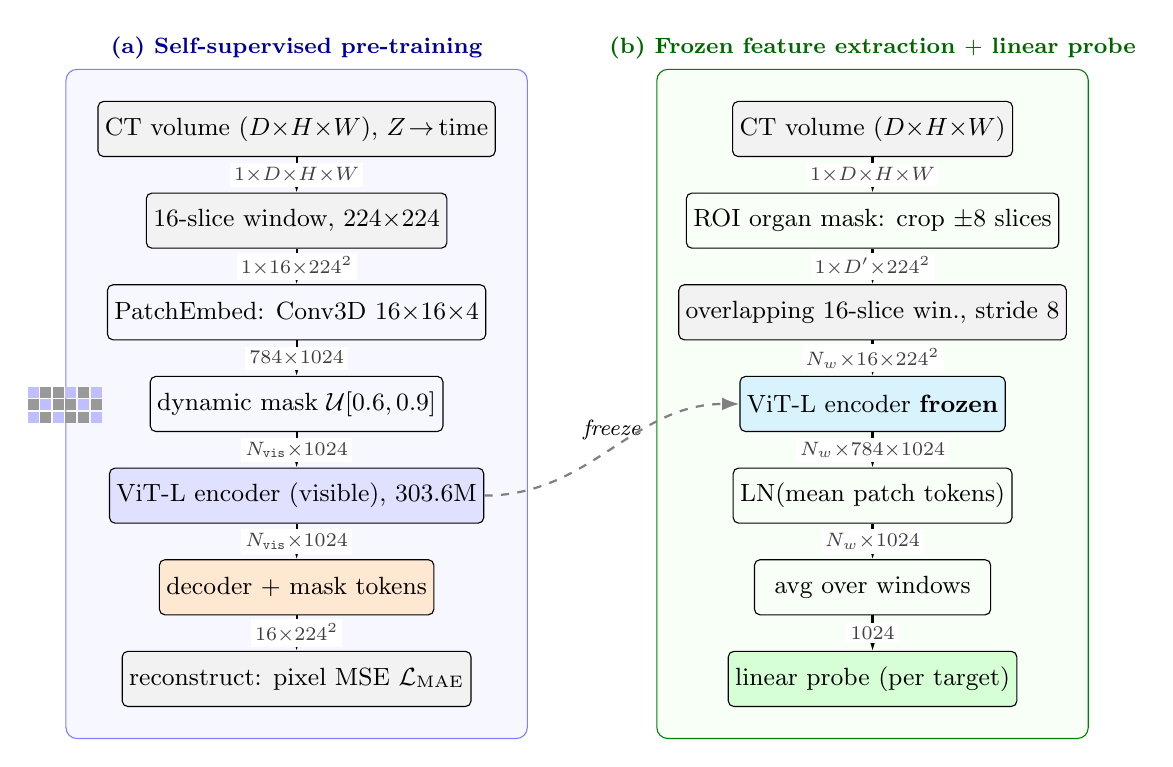
\begin{tikzpicture}[
  font=\small,
  >={Latex[length=2.2mm]},
  node distance=4.5mm and 30mm,
  block/.style={draw, rounded corners=2pt, align=center, minimum height=7mm,
                minimum width=30mm, inner sep=2.5pt},
  data/.style={block, fill=black!5},
  enc/.style={block, fill=blue!12},
  dec/.style={block, fill=orange!18},
  frozen/.style={block, fill=cyan!15},
  head/.style={block, fill=green!16},
  lbl/.style={font=\footnotesize\itshape},
  dim/.style={font=\scriptsize\ttfamily, text=black!75, fill=white,
              inner sep=1.5pt},
  arr/.style={->, thick}
]

% ========== Lane (a): self-supervised pre-training (top-down) ==========
\node[data] (vol) {CT volume $(D{\times}H{\times}W)$, $Z\!\to\!$ time};
\node[data, below=of vol]  (win)  {$16$-slice window, $224{\times}224$};
\node[block, below=of win] (pe)   {PatchEmbed: Conv3D $16{\times}16{\times}4$};
\node[block, below=of pe]  (mask) {dynamic mask $\mathcal{U}[0.6,0.9]$};
\node[enc, below=of mask]  (enc)  {ViT-L encoder (visible), $303.6$M};
\node[dec, below=of enc]   (dec)  {decoder $+$ mask tokens};
\node[data, below=of dec]  (rec)  {reconstruct: pixel MSE $\mathcal{L}_{\text{MAE}}$};

\draw[arr] (vol)--(win)   node[dim,midway]{$1{\times}D{\times}H{\times}W$};
\draw[arr] (win)--(pe)    node[dim,midway]{$1{\times}16{\times}224^2$};
\draw[arr] (pe)--(mask)   node[dim,midway]{$784{\times}1024$};
\draw[arr] (mask)--(enc)  node[dim,midway]{$N_{\text{vis}}{\times}1024$};
\draw[arr] (enc)--(dec)   node[dim,midway]{$N_{\text{vis}}{\times}1024$};
\draw[arr] (dec)--(rec)   node[dim,midway]{$16{\times}224^2$};

% small masked-token grid left of the mask node (grey = masked, blue = visible)
\begin{scope}[shift={($(mask.west)+(-1.55,-0.24)$)}]
  \foreach \x in {0,...,5}{
    \foreach \y in {0,...,2}{
      \pgfmathtruncatemacro{\m}{mod(\x*2+\y*3+\x,5)>1 ? 1 : 0}
      \ifnum\m=1
        \fill[black!40] (\x*0.16,\y*0.16) rectangle ++(0.14,0.14);
      \else
        \fill[blue!25] (\x*0.16,\y*0.16) rectangle ++(0.14,0.14);
      \fi
    }
  }
\end{scope}

% ========== Lane (b): frozen feature extraction + linear probe ==========
\node[data, right=of vol]   (vol2) {CT volume $(D{\times}H{\times}W)$};
\node[block, below=of vol2] (roi)  {ROI organ mask: crop $\pm8$ slices};
\node[data, below=of roi]   (winN) {overlapping $16$-slice win., stride $8$};
\node[frozen, below=of winN](enc2) {ViT-L encoder \textbf{frozen}};
\node[block, below=of enc2] (pool) {LN(mean patch tokens)};
\node[block, below=of pool] (avg)  {avg over windows};
\node[head, below=of avg]   (lp)   {linear probe (per target)};

\draw[arr] (vol2)--(roi)   node[dim,midway]{$1{\times}D{\times}H{\times}W$};
\draw[arr] (roi)--(winN)   node[dim,midway]{$1{\times}D'{\times}224^2$};
\draw[arr] (winN)--(enc2)  node[dim,midway]{$N_w{\times}16{\times}224^2$};
\draw[arr] (enc2)--(pool)  node[dim,midway]{$N_w{\times}784{\times}1024$};
\draw[arr] (pool)--(avg)   node[dim,midway]{$N_w{\times}1024$};
\draw[arr] (avg)--(lp)     node[dim,midway]{$1024$};

% reuse of pretrained weights: encoder (a) -> frozen encoder (b)
\draw[->, thick, dashed, gray] (enc.east) to[out=0,in=180]
      node[midway,above,lbl,black]{freeze} (enc2.west);

% ========== background panels with stage labels ==========
\begin{scope}[on background layer]
  \node[draw=blue!50, rounded corners, fill=blue!3, inner sep=4mm,
        fit=(vol)(rec), label={[font=\bfseries\footnotesize,blue!60!black]
        above:(a) Self-supervised pre-training}] {};
  \node[draw=green!50!black, rounded corners, fill=green!3,
        inner xsep=9mm, inner ysep=4mm,
        fit=(vol2)(lp), label={[font=\bfseries\footnotesize,green!40!black]
        above:(b) Frozen feature extraction $+$ linear probe}] {};
\end{scope}

\end{tikzpicture}%
}
\caption{Pipeline; tensor shapes on each arrow trace the data transformation
(channel-first; $N_{\text{vis}}$ visible tokens after masking, $N_w$ stride-$8$
windows, $D'$ cropped depth). \textbf{(a) Pre-training:} a CT volume is treated as
a video ($Z\!\to\!$ time); a random $16$-slice window at $224^2$ is patch-embedded
with a $16{\times}16$ spatial / $4$-slice temporal kernel into
$4{\times}14{\times}14{=}784$ tokens of width $1024$, a dynamic fraction
($60$--$90\%$, grey squares) is masked, the ViT-Large encoder sees only the
$N_{\text{vis}}$ visible tokens (blue squares), and a lightweight decoder
reconstructs the masked voxels under a pixel-MSE loss. \textbf{(b) Feature
extraction (frozen):} the trained encoder is frozen; a volume is tiled into $N_w$
overlapping $16$-slice windows (stride $8$), each window yields a
layer-normalized patch-token mean ($N_w{\times}1024$), and the per-window vectors
are averaged into a single $1024$-d descriptor on which the organizers train a
linear probe. For the eleven ROI targets the volume is first cropped to the
provided organ mask ($\pm8$ context slices).}
\label{fig:Network}
\end{figure}

\subsection{Self-supervised pre-training}

\paragraph{CT-as-video formulation.}
A CT volume of shape $(D,H,W)$ is normalized (Sec.~\ref{sec:preproc}) and a
contiguous window of $T{=}16$ axial slices is resized to $16{\times}224{\times}224$
and treated as a single-channel ($C{=}1$) clip. A 3D patch-embedding convolution
with spatial kernel $16{\times}16$ and \emph{temporal kernel $4$} (stride equal
to kernel) produces a token grid of size $(T/4)\times(H/16)\times(W/16)=
4{\times}14{\times}14=784$ tokens of dimension $1024$, to which a learnable
class token and \emph{separable} spatial/temporal positional embeddings are
added.
Because we adopt MAE-ST's spacetime-\emph{agnostic random} masking, our pretext
task is, in effect, identical to randomly masking 3D patches of a volume:
whether the third axis is labelled ``depth'' or ``time'' does not change the
token set or the masking distribution. We therefore make no claim that a video
formulation \emph{per se} differs from a native volumetric MAE. What
distinguishes our backbone from the volumetric 3D MAEs common in medical imaging
is inherited from the video model along two concrete axes: (i) \emph{anisotropic
patch embedding} -- a $16{\times}16$ in-plane patch but a coarser temporal patch
of $4$ slices, tokenizing the through-plane ($Z$) axis at a different granularity
than a cubic $16^3$ patch; and (ii) \emph{factorized} (separable) spatial and
temporal positional embeddings rather than a single joint 3D embedding. We
additionally depart from the prevailing fine-tuned-segmentation protocol by
evaluating the encoder strictly \emph{frozen} under linear probing.

\paragraph{Masked reconstruction.}
Following MAE~\cite{mae,maest}, on each forward pass we sample a masking ratio
$r\sim\mathcal{U}[0.6,0.9]$ and randomly drop a fraction $r$ of the $784$ tokens.
The ViT-Large \emph{encoder} ($24$ blocks, $1024$-d, $16$ heads,
mlp-ratio $4$) processes only the visible tokens. An asymmetric
\emph{decoder} ($8$ blocks, $512$-d, $16$ heads) receives the encoded visible
tokens plus shared mask tokens and reconstructs the masked content; the loss is
the mean-squared error between predicted and ground-truth voxels, computed
\emph{only over masked patches} (raw-pixel target, no per-patch normalization):
\[
\mathcal{L}_{\text{MAE}}
= \frac{1}{|\mathcal{M}|}\sum_{i\in\mathcal{M}}\big\lVert \hat{x}_i - x_i \big\rVert_2^2 ,
\]
where $\mathcal{M}$ indexes masked patches. The temporal prediction dimension is
$16$, so the decoder reconstructs all $16$ input slices.

\paragraph{Why dynamic masking.}
The encoder sees $\lfloor 784\,(1-r)\rfloor$ tokens, so a fixed high ratio
(e.g.\ $90\%$) leaves only $78$ visible tokens and makes \emph{every} iteration
maximally hard. Sampling $r\sim\mathcal{U}[0.6,0.9]$ independently each step
instead exposes the encoder to a range of reconstruction difficulties -- from
$313$ visible tokens ($60\%$, rich context) to $78$ ($90\%$, aggressive
inpainting), a $4\times$ spread in available context -- within a single training
run, rather than committing to one fixed difficulty. The sampling distribution
is stationary across training, so this is difficulty \emph{mixing} rather than a
scheduled easy-to-hard curriculum. This is consistent with recent evidence that
exposing a masked autoencoder to a \emph{range} of masking ratios, rather than a
single fixed value, encourages multi-scale feature learning and can surpass even
the best-tuned fixed ratio~\cite{r2mae}. That evidence is our motivation for
adopting dynamic masking, not evidence about our own encoder: our ablation
changes this setting together with ten others (Sec.~\ref{sec:ablation}), so we
cannot quantify its individual contribution here and do not claim one.

\paragraph{Backbone details.}
ViT-Large, patch $16{\times}16$ (spatial) $\times\,4$ (temporal), embedding
dimension $1024$, depth $24$, $16$ heads, mlp-ratio $4$, separable
spatio-temporal position embeddings and a class token. The frozen encoder loaded
at inference has \textbf{$303.6$\,M parameters} (decoder and mask tokens are
stripped from the checkpoint and are not shipped in the container).

\subsection{Inference: frozen feature extraction and linear probing}
\label{sec:inference}
At inference the decoder is discarded and the encoder is frozen; the system maps
a full-resolution, arbitrary-depth CT volume to a single descriptor that the
organizers' linear probe then classifies.

\paragraph{Global feature from the frozen backbone.}
Given a single $16$-slice
window, we run the frozen encoder \emph{without} masking, drop the class token, take the
\emph{mean over the $784$ patch tokens}, and apply the final encoder
LayerNorm, yielding a $1024$-d vector. We chose mean-pooled patch tokens over the
class token because, under a reconstructive objective, the class token is never
supervised, whereas patch tokens directly carry localized anatomical evidence.

\paragraph{Windowed aggregation for arbitrary-depth volumes.}
\label{sec:agg}
Clinical CTs have variable depth $D$ (tens to hundreds of slices), but the
encoder consumes exactly $16$ slices. We therefore slide a $16$-slice window
along Z with \textbf{stride $8$ ($50\%$ overlap)}, resize each window in-plane to
$224^2$ by trilinear interpolation, and \emph{average} the per-window $1024$-d
descriptors into one volume-level vector. Windows are emitted at
$z=0,8,16,\dots$ for as long as $z+16\le D$; if the last such window does not
reach the final slice, we append one additional window \emph{shifted} to occupy
$[D-16,\,D)$. The tail window is therefore anchored to the end of the volume and
simply overlaps its predecessor by more than $8$ slices -- no zero- or
edge-padding is used, and no slice is dropped. Padding is applied only in the
degenerate case $D<16$, where the volume is extended to $16$ slices by
replicating its last slice (\texttt{mode=edge}). Overlapping windows make the
descriptor robust to where structures fall relative to window boundaries. Rather than encoding one window at a time, we stack $8$
windows into a single GPU batch, which uses the device far more efficiently and
speeds up per-case feature extraction.

\paragraph{ROI versus non-ROI targets.}
Eleven targets are ROI-based (organ-specific): for these the organizers provide a
foreground organ mask, and we restrict feature extraction to the masked
sub-volume; the remaining targets are treated globally (whole-volume descriptor).
For an ROI target we read the provided mask, find the Z-range where the mask is
active, expand it by $\pm 8$ context slices, crop the volume to that range, and
then apply the same windowed aggregation. This focuses the descriptor on the
organ of interest (e.g.\ adrenal gland for \emph{adrenal\_hyperplasia}) while
retaining peri-organ context. If the padded mask range spans fewer than $16$
slices, it is re-centred on its own midpoint and widened to exactly $16$ slices
(clipped to the volume), so that at least one full window is always available.
Cropping also leaves fewer $16$-slice windows to pass through the ViT, which
lowers per-case compute and runtime. If a mask is empty we fall back to the
global descriptor.

\paragraph{Linear-probe head.}
The container emits only frozen $1024$-d features; per challenge protocol, the
\emph{organizers} fit the linear probe. For internal model selection we
replicate the standard LP recipe: $L_2$-normalize each descriptor and fit a
per-target $\ell_2$-regularized logistic regression with
\emph{class-balanced} weighting (to counter the severe positive/negative
imbalance), sweeping the inverse regularization strength
$C\in\{10^{-3},10^{-2},10^{-1},1,10,10^{2}\}$. Balanced accuracy is computed by
thresholding the predicted positive probability at $0.5$; because the
organizer-provided validation split is exactly class-balanced
(Sec.~\ref{sec:data}), balanced accuracy there coincides with plain accuracy.

Two properties of this internal recipe must be stated plainly, because they bound
how the numbers in Sec.~\ref{sec:valres} should be read. First, $C$ is selected
\emph{by validation AUROC on the same split that we then report}, and the
checkpoint (Sec.~\ref{sec:protocols}) is selected the same way; we did not hold
out a separate split or use nested cross-validation. The reported per-target
values are therefore selection-optimistic upper bounds rather than unbiased
estimates of held-out performance, and the bias is largest for the targets with
the smallest $n_\text{val}$ ($52$--$266$ cases). Second, the official score is
produced by the organizers' own probe on their own split, not by this recipe;
ours exists only to rank our candidate checkpoints. Sec.~\ref{sec:valtest}
quantifies how much of the validation-to-test difference this optimism can
account for. A linear probe has no capacity to compensate for a weak backbone,
which is exactly why it is a faithful probe of feature quality.

% ======================================================================
\section{Experiments}

\subsection{Dataset and evaluation metrics}
\label{sec:data}
The challenge provides a large-scale unlabeled CT pre-training set and a
downstream train/validation set of \textbf{$17$ binary classification targets
across three datasets}, spanning abdomen and chest. For Task~1 we enter the
\textbf{All-Data track}, pre-training from scratch on the full corpus. Our
\emph{internal} validation pipeline covers the $15$ abdominal (AMOS-derived)
targets -- $11$ ROI and $4$ non-ROI; the two additional official targets are
chest findings (a COVID-CT target and a lung-nodule-malignancy target) that are
absent from our local split, so all internally reported per-disease numbers are
\emph{abdominal}.

\paragraph{Train/validation split.}
We did not construct the split. Each target ships as a per-target label CSV with
a \texttt{case\_id}, a binary label and a \texttt{split} column, and we use that
\texttt{train}/\texttt{val} partition verbatim; no case is moved, resampled or
re-stratified, and no pre-training volume appears in it (pre-training uses the
separate unlabeled corpus). The partition is target-specific, so the number of
cases differs per target: $576$--$1107$ training and $52$--$266$ validation cases
(the $n_\text{val}$ column of Table~\ref{tab:results-lp}). Two properties of this
partition matter for interpreting our numbers. The \emph{validation} partition is
exactly class-balanced -- precisely $50\%$ positives for all $15$ targets, by
construction of the released split -- which is why we describe it as the
``class-balanced AMOS-15'' split and why balanced accuracy equals accuracy there.
The \emph{training} partition instead carries the natural prevalence, ranging
from $6.4\%$ positives (splenomegaly) to $50\%$ (liver cyst, renal cyst); this is
the imbalance that the class-balanced logistic-regression weighting is there to
counter.

\noindent\textbf{Classification metrics.}
\emph{Balanced accuracy} (mean of sensitivity and specificity), robust to
imbalance, and \emph{AUROC}. \textbf{Efficiency metric:} per-case running time
in seconds, including container start-up; for Task~1 this is the average
feature-extraction time per target.

\subsection{Implementation details}

\subsubsection{Preprocessing.}
\label{sec:preproc}
Each NIfTI volume is loaded and transposed to $(D,H,W)$ with $Z$ first. Hounsfield
units are clipped to $[-1024, 3071]$ and linearly mapped to $[0,1]$; this single
fixed window is used at both pre-training and inference, so train/test
preprocessing is identical. During pre-training a random contiguous $16$-slice
window is drawn (short volumes are tiled to reach $16$ slices) and resized
in-plane to $224^2$ by trilinear interpolation. At inference the deterministic
overlapping-window scheme of Sec.~\ref{sec:agg} replaces the random crop. For
fast large-scale loading we read NIfTI arrays lazily via memory-mapped
\texttt{dataobj} access and apply all augmentation on the fly on $(1,T,H,W)$
tensors; no resampling to isotropic spacing is performed, which avoids an
expensive global resample on every volume.

\subsubsection{Environment settings.}
Development and runtime environments are summarized in Table~\ref{table:env}.

\begin{table}[!htbp]
\caption{Development environments and requirements.}\label{table:env}
\centering
\begin{tabular}{ll}
\hline
System            & Ubuntu 20.04 LTS (kernel 5.4.0) \\ \hline
CPU               & Intel Xeon Gold 6130 @ $2.10$\,GHz ($2{\times}16$ cores, $64$ threads) \\ \hline
RAM (pre-training)& $96$\,GB (Slurm allocation) \\ \hline
RAM (inference)   & container limit $32$\,GB (\texttt{-m 32G}) \\ \hline
GPU (pre-training)& $3\times$ NVIDIA Titan RTX $24$\,GB \\ \hline
GPU (inference)   & $1\times$ NVIDIA GPU (\texttt{--gpus device=0}) \\ \hline
CUDA version      & $12.1$ \\ \hline
Programming language & Python $3.9$ \\ \hline
Deep learning framework & PyTorch $2.1.0$ \\ \hline
Key libraries     & nibabel, h5py, timm, iopath, numpy \\ \hline
\end{tabular}
\end{table}

\subsubsection{Training protocols.}
\label{sec:protocols}
\textbf{(1) Data augmentation.} During pre-training, augmentations are applied
consistently across all $16$ slices of a clip: random horizontal flip ($p{=}0.5$),
vertical flip ($p{=}0.5$), random $90/180/270^{\circ}$ axial rotation, random
intensity scale $\mathcal{U}[0.95,1.05]$ and shift $\mathcal{U}[-0.05,0.05]$, and
additive Gaussian noise ($p{=}0.3$, $\sigma{=}0.02$), with values re-clamped to
$[0,1]$. Inference uses no augmentation (no test-time augmentation).
\textbf{(2) Sampling.} Each epoch draws one random $16$-slice window per volume
(random start index), giving stochastic depth coverage across epochs.
Repeat-augmentation ($\times4$) replicates each sampled clip into four
independently augmented views per iteration, so an optimizer step sees $96$
augmented samples spanning the $24$ unique clips of the effective batch.
\textbf{(3) Stopping criterion.} There was none in the usual sense: no
validation signal was used to stop pre-training, because the pretext objective
is unsupervised and no downstream labels enter the pre-training loop. The run was
scheduled for $250$ epochs with a checkpoint written every $10$ epochs, and was
stopped manually after epoch $134$ once the epoch-mean masked-patch MSE had been
flat for ${\sim}50$ epochs ($8.6$--$9.0\times10^{-4}$, Fig.~\ref{fig:curve}
inset) and the remaining challenge compute budget was better spent on
feature extraction. The schedule was therefore truncated, not completed: the
cosine decay was still at $5.4\times10^{-5}$ rather than $0$ when the run ended,
so the final checkpoint is a converged-plateau checkpoint and not a
fully-annealed one.
\textbf{(4) Checkpoint selection.} The two checkpoints we evaluated were epoch
$40$, which is exactly the end of the $40$-epoch linear warm-up and the earliest
point at which the learning rate has peaked, and epoch $130$, the last
checkpoint written before the run was stopped. We extracted features for both and
selected by internal validation mean AUROC; epoch $130$ won and was submitted.
We did not sweep the intermediate checkpoints, so epoch $130$ is the better of
two candidates rather than an optimum over the thirteen available. Note also
that this selection uses the same split that Table~\ref{tab:results-lp} reports,
and contributes to the optimism discussed in Sec.~\ref{sec:inference}; the
epoch-$40$ checkpoint scores $0.646$ mean AUROC on this split, against $0.678$ at
epoch $130$ (Sec.~\ref{sec:ablation}).

Table~\ref{table:training-lp} gives the full pre-training and linear-head
protocol.
Figure~\ref{fig:curve} shows the pre-training reconstruction loss and learning-rate
schedule: the masked-patch MSE drops sharply within the first few epochs and then
decreases smoothly, while the learning rate follows the $40$-epoch linear warm-up
to $9.4\times10^{-5}$ and the subsequent cosine decay. The submitted checkpoint
(epoch $130$) sits on the converged plateau.

\begin{figure}[!t]
\centering
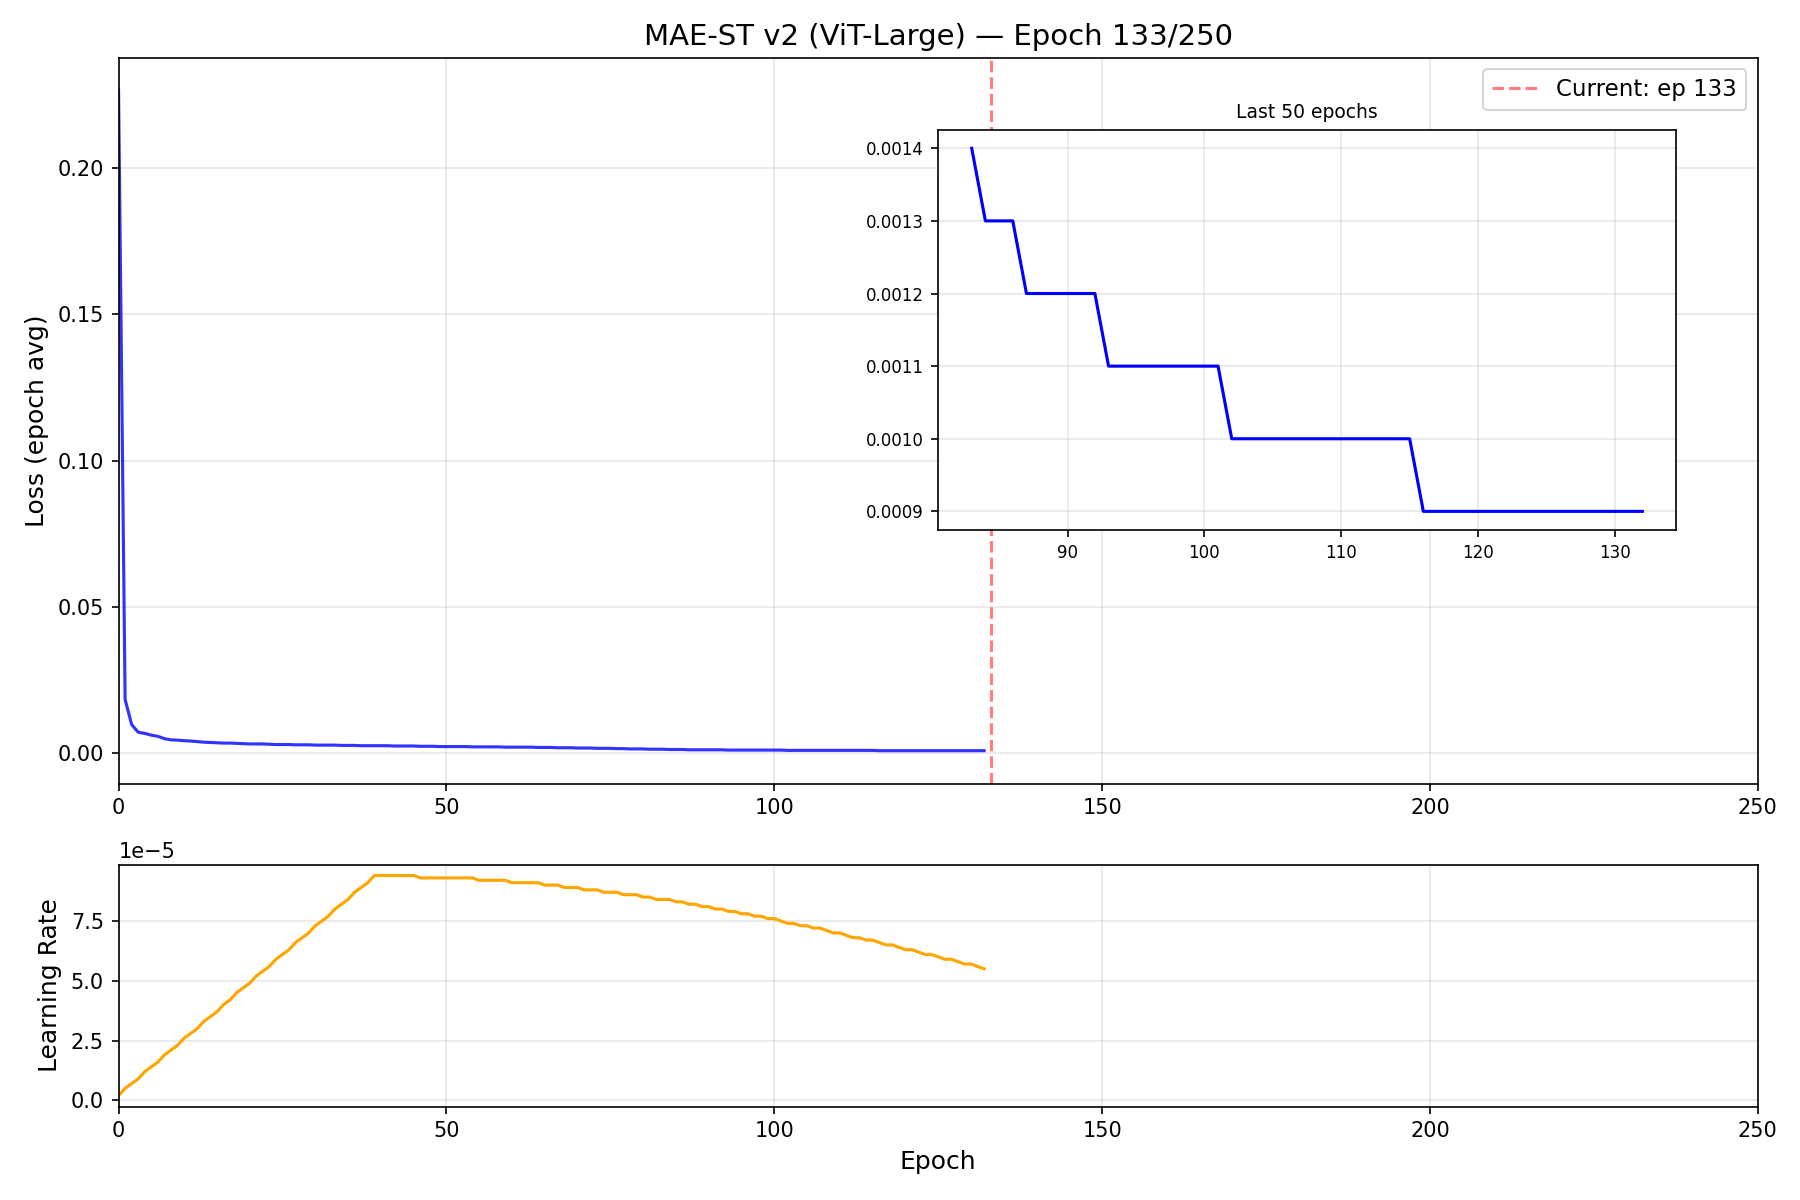
\includegraphics[width=\textwidth]{imgs/maest_v2_training_curve.png}
\caption{MAE-ST (ViT-Large) pre-training. \textbf{Top:} per-epoch masked-patch
reconstruction loss (inset: last $50$ epochs, $\sim\!9\times10^{-4}$); the dashed
line marks the submitted epoch-$130$ checkpoint. \textbf{Bottom:} the per-epoch
learning rate -- linear warm-up over $40$ epochs to $9.4\times10^{-5}$ followed by
cosine decay (linear-scaling rule, effective batch $24$). Training ran to
epoch $134$ of $250$ scheduled and was stopped on the converged plateau
(Sec.~\ref{sec:protocols}); the last checkpoint written was epoch $130$. Axes
are cropped to the trained range.}
\label{fig:curve}
\end{figure}

\begin{table*}[!htbp]
\caption{Training protocols for Task~1 -- Linear Probing (pre-training and
linear-head training).}
\label{table:training-lp}
\begin{center}
\begin{tabular}{ll}
\hline
Pre-trained backbone (if any)   & None -- MAE-ST pre-trained from scratch (All-Data) \\ \hline
Backbone tuning strategy        & Frozen \\ \hline
Batch size (pre-training)       & $24$ effective ($4$/GPU $\times\,2$ accum $\times\,3$ GPU) \\ \hline
Patch / volume size             & input $16\times224\times224$; patch $16\times16\times4$ \\ \hline
Total pre-training epochs       & $250$ sched.; stopped at $134$; ep.\ $130$ submitted \\ \hline
Linear-head epochs              & Logistic regression, $C$-sweep (6 values), no SGD epochs \\ \hline
Optimizer                       & AdamW ($\beta=0.9,0.95$), weight decay $0.05$ \\ \hline
Initial learning rate (lr)      & $9.4\times10^{-5}$ (blr $10^{-3}\times24/256$) \\ \hline
Lr decay schedule               & $40$-ep.\ linear warmup, cosine (truncated at ep.\ $134$) \\ \hline
Pre-training time               & $\approx 65.8$ hours ($1$ node, $3\times$ Titan RTX) \\ \hline
Linear-head training time       & $<1$ min/target (logistic regression) \\ \hline
Loss function                   & Masked-patch pixel MSE \\ \hline
Number of model parameters      & $303.6$\,M (frozen encoder) \\ \hline
\end{tabular}
\end{center}
\end{table*}

\subsection{Quantitative results on the validation set}
\label{sec:valres}

\paragraph{Validation performance.}
Under the frozen-LP protocol, MAE-ST attains a validation \textbf{mean AUROC of
$0.678$} (mean balanced accuracy $0.638$) over the $15$ AMOS abdominal targets.
This figure is higher than the $17$-target \emph{test} AUROC ($0.624$,
Sec.~\ref{sec:test}), and it should be read as a selection-optimistic internal
estimate rather than as a prediction of test performance: both the checkpoint and
the per-target $C$ were chosen on this split (Sec.~\ref{sec:inference}), and the
split differs from the official test set in both composition and anatomy.
Sec.~\ref{sec:valtest} decomposes the difference; under plausible assumptions
the two unseen chest targets account for less than half of it.

\paragraph{Per-disease validation detail.}
Table~\ref{tab:results-lp} reports per-target AUROC and balanced accuracy on the
class-balanced AMOS-15 validation set (epoch-130 submitted checkpoint). The
per-target dynamic range is large ($0.587\!\to\!0.841$ AUROC), which the mean
hides: the strongest targets are organ-scale, high-contrast findings
(splenomegaly, fatty liver), while the weakest are focal/cystic findings
(liver cyst, liver calcifications, gallstone). Aggregated by region of interest,
ROI and non-ROI targets are nearly tied ($0.685$ vs.\ $0.660$ mean AUROC).

\begin{table}[htbp]
\caption{Task~1 LP \textbf{All-Data}, \textbf{validation set}. Per-disease AUROC
and balanced accuracy on the organizer-provided, exactly class-balanced AMOS-15
validation split (MAE-ST, epoch-130 submitted checkpoint; $303.6$\,M params).
Targets sorted by AUROC; $n_\text{val}$ is the number of validation cases, of
which exactly half are positive. \emph{These are selection-optimistic values,
not held-out estimates}: the checkpoint and the per-target $C$ were both chosen
by AUROC on this same split (Sec.~\ref{sec:inference}), with no separate
held-out split, no nested cross-validation and no confidence intervals. Balanced
accuracy is at a fixed $0.5$ probability threshold and, on a balanced split,
equals accuracy.}
\label{tab:results-lp}
\centering
\begin{tabular}{llccc}
\hline
Target & Type & AUROC & BalAcc & $n_\text{val}$ \\ \hline
splenomegaly         & ROI     & \textbf{0.841} & 0.729 & 70  \\ \hline
fatty\_liver          & ROI     & 0.825 & 0.679 & 78  \\ \hline
cholecystitis        & ROI     & 0.727 & 0.706 & 102 \\ \hline
adrenal\_hyperplasia  & ROI     & 0.713 & 0.686 & 70  \\ \hline
colorectal\_cancer    & non-ROI & 0.695 & 0.673 & 52  \\ \hline
hydronephrosis       & ROI     & 0.692 & 0.703 & 64  \\ \hline
lymphadenopathy      & non-ROI & 0.677 & 0.625 & 72  \\ \hline
kidney\_stone         & ROI     & 0.676 & 0.633 & 158 \\ \hline
ascites              & non-ROI & 0.655 & 0.647 & 68  \\ \hline
renal\_cyst           & ROI     & 0.639 & 0.605 & 266 \\ \hline
liver\_lesion         & ROI     & 0.620 & 0.522 & 134 \\ \hline
atherosclerosis      & non-ROI & 0.612 & 0.603 & 68  \\ \hline
gallstone            & ROI     & 0.607 & 0.612 & 116 \\ \hline
liver\_calcifications & ROI     & 0.603 & 0.569 & 72  \\ \hline
liver\_cyst           & ROI     & 0.587 & 0.578 & 244 \\ \hline
\textbf{All AMOS-15}  &         & \textbf{0.678} & \textbf{0.638} & 15 \\ \hline
ROI ($11$)           &         & 0.685 & 0.638 & 11 \\ \hline
non-ROI ($4$)        &         & 0.660 & 0.637 & 4  \\ \hline
\end{tabular}
\end{table}

\subsection{Ablation study}
\label{sec:ablation}

\paragraph{Submitted recipe vs.\ an earlier configuration.}
Table~\ref{tab:ablation} compares the submitted MAE-ST recipe against our
earlier internal configuration (``v1''). This is a \emph{recipe-level} comparison
and nothing finer: the two runs differ in \textbf{eleven} settings simultaneously,
enumerated in the lower panel of Table~\ref{tab:ablation}, spanning the masking
distribution, the tokenization and temporal prediction target, the decoder, the
reconstruction target, the optimizer schedule and gradient clipping, the training
length, the effective batch size and the augmentation pipeline (including
repeated augmentation). Both runs pre-train on the identical set of
$10{,}819$ volumes, so the training data is not among the differences.
The full recipe gains $+0.051$ AUROC ($0.627 \to 0.678$), improving $12$ of $15$
targets. The largest per-target gains are on organ-scale findings: splenomegaly
$0.663\!\to\!0.841$ ($+0.178$), liver calcifications $0.440\!\to\!0.603$
($+0.163$, rescued from below chance), and atherosclerosis
$0.493\!\to\!0.612$ ($+0.119$, raised above chance).

We want to be explicit about what this comparison does \emph{not} establish.
Because eleven settings move together -- including training length ($100$
epochs versus $134$ of a $250$-epoch schedule), the base learning rate, the
warm-up length, the reconstruction target and the gradient-clipping threshold, each of which alone can move a frozen-feature mean AUROC -- the
experiment licenses only the aggregate statement that the submitted recipe is
better than v1 by $0.051$ on this split. It licenses no statement about dynamic
masking, about the coarse temporal patch, or about any other individual setting,
and the $+0.051$ should not be read as the effect of the design choices
highlighted in the abstract and in Sec.~\ref{sec:intro-contrib}. Single-factor
runs -- at minimum fixed $0.9$ versus $\mathcal{U}[0.6,0.9]$ and $t_p{=}2$ versus
$t_p{=}4$ on a short, matched schedule -- are what would be needed, and they
did not fit the challenge timeline (Sec.~\ref{sec:limitations}). For context, the
epoch-$40$ checkpoint of the submitted run scores $0.646$, between v1 ($0.627$)
and the submitted epoch $130$ ($0.678$). This does not isolate training length
either: because of the smaller effective batch and $\times4$ repeated
augmentation, the submitted run has already taken more optimizer steps
(${\approx}18$k vs.\ ${\approx}11$k) and processed more augmented samples
(${\approx}1.7$M vs.\ ${\approx}1.1$M) by epoch $40$ than v1 did in its entire
run, and the further $+0.032$ from epoch $40$ to $130$ is confounded with the
learning-rate schedule (epoch $40$ is the warm-up peak).

% ----------------------------------------------------------------------
% ABLATION TABLE SOURCE. Both columns are read from the args saved inside
% the checkpoints: v1 = job 15124346, checkpoints/ct_maest_pretrain/
% checkpoint-00099.pth (12 GPUs); v2 = job 15326473 (3 GPUs). Both runs use
% a class token and FP32, so those are NOT differences. v1 augmentation
% (h-flip only) verified from the v1 mae_st/dataset_ct_maest.py (2026-03-09);
% v2 from mae_st_v2/dataset_ct_maest.py (2026-03-17). The two runs' file lists
% (train_files.txt, flare_train_files.txt) are byte-identical: same 10,819
% FLARE volumes, so pre-training data is NOT a difference.
% ----------------------------------------------------------------------
\begin{table}[htbp]
\caption{Recipe-level ablation: submitted MAE-ST recipe vs.\ our earlier
configuration ``v1'' (AMOS-15 internal validation, mean AUROC). The lower panel
enumerates \emph{all eleven} settings in which the two runs differ. Because they
move together, this table attributes the $+0.051$ to the recipe as a whole and
to no individual row; per-setting attribution requires one-change-at-a-time runs
(Sec.~\ref{sec:limitations}).}\label{tab:ablation}
\centering
\begin{tabular}{lc}
\hline
Configuration & Mean AUROC \\ \hline
MAE-ST v1 (earlier configuration)   & $0.627$ \\
\textbf{MAE-ST submitted (ep130)}   & $\mathbf{0.678}$ \\
\textbf{Difference}                 & $\mathbf{+0.051}$ \\ \hline
\end{tabular}

\vspace{1.2ex}
\begin{tabular}{llll}
\hline
\# & Setting & v1 & Submitted \\ \hline
1  & Mask ratio            & fixed $0.9$              & $\mathcal{U}[0.6,0.9]$ per step \\
2  & $t_p$ / predicted slices & $2$ / $8$ ($1568$ tokens) & $4$ / $16$ ($784$ tokens) \\
3  & Decoder depth         & $4$ blocks               & $8$ blocks \\
4  & Loss target           & per-patch normalized     & raw pixels \\
5  & Base lr (blr)         & $1.5{\times}10^{-4}$     & $10^{-3}$ \\
6  & Warm-up               & $10$ epochs              & $40$ epochs \\
7  & Scheduled epochs      & $100$ (completed)        & $250$ (stopped at $134$) \\
8  & Gradient clipping     & $0.02$                   & $1.0$ \\
9  & Augmentation          & h-flip only              & flips, rot., intensity, noise \\
10 & Repeated augmentation & $\times1$               & $\times4$ \\
11 & Effective batch       & $96$ ($12$ GPU)          & $24$ ($3$ GPU) \\ \hline
\end{tabular}
\end{table}

\paragraph{Aggregation and ROI cropping (design rationale).}
Two further design choices were guided by informal internal checks that we did
not record quantitatively; we summarize the rationale here and make no
performance claim for either.
\emph{(i) Multi-window overlap.} Overlapping ($50\%$) windows with mean pooling
appeared more stable than non-overlapping windows, particularly for findings that can
fall between window boundaries.
\emph{(ii) ROI cropping.} For the eleven ROI targets, mask-guided cropping
(organ range $\pm 8$ slices) concentrates the descriptor on the relevant organ
and reduces runtime by shrinking the window list. We did not run a head-to-head
comparison against whole-volume features, so we make no discrimination claim;
ROI and non-ROI targets in fact reach comparable validation AUROC
($0.685$ vs.\ $0.660$).

\subsection{Results on the final testing set}
\label{sec:test}
Table~\ref{tab:leaderboard} reports the official final-test ranking for the
Task~1 LP All-Data track. Our team (\textbf{maest}) places $4^{\text{th}}$ on the
published leaderboard (top six shown)
with $0.600$ balanced accuracy and $0.624$ AUROC at $6.27$\,s/case -- the
third-fastest runtime among the top four (behind raidium at $4.39$\,s and cemrg
at $4.47$\,s, ahead of fomofo at $9.41$\,s) and roughly $5\times$ faster than the
slowest valid entry. The leading cluster (fomofo / raidium / cemrg) sits at
$0.705$--$0.714$ AUROC, $0.08$--$0.09$ above ours. Cross-region (chest)
generalization is unlikely to be the whole explanation: Sec.~\ref{sec:valtest}
estimates that most of our own validation-to-test drop comes from the abdominal
targets.

\begin{table}[htbp]
\caption{Official final-test ranking, Task~1 LP \textbf{All-Data} track ($17$
targets). Our submission is \textbf{maest}. Runtime is seconds per case including
container start-up.}\label{tab:leaderboard}
\centering
\begin{tabular}{clccc}
\hline
Rank & Team & Balanced Acc & AUROC & Runtime (s) \\ \hline
1 & fomofo            & 0.654 & 0.714 & 9.414 \\
2 & raidium           & 0.639 & 0.707 & 4.393 \\
3 & cemrg             & 0.643 & 0.705 & 4.467 \\
\textbf{4} & \textbf{maest (ours)} & \textbf{0.600} & \textbf{0.624} & \textbf{6.273} \\
5 & xupy              & 0.566 & 0.599 & 10.860 \\
6 & sdfmu             & 0.160 & 0.170 & 33.830 \\ \hline
\end{tabular}
\end{table}

\subsection{Accounting for the validation-to-test difference}
\label{sec:valtest}
Our internal estimate ($0.678$ over $15$ abdominal targets) and the official
score ($0.624$ over $17$) differ by $0.054$ AUROC. It is tempting to charge the
whole difference to the two chest targets our encoder never saw. The arithmetic
does not support it.

We take the official score to be an unweighted mean over the $17$ targets. The
aggregation rule is not stated in the public challenge materials: the released
evaluation code computes the metrics for each target independently and writes
one row per target without combining
them,\footnote{\url{https://github.com/kmin940/CVPR26-3DCTFMCompetition}
(\nolinkurl{cvpr26_eval_metrics-dev.py},
\nolinkurl{cvpr26_organize_eval_metrics_and_predictions.py}); the leaderboard
scoring program is not published.} while the leaderboard reports a single
balanced accuracy and AUROC per team, so the per-target values must be averaged
somewhere in the scoring program. A macro mean over targets is the reading
consistent with that code's per-target structure, but it is an assumption. The
qualitative conclusion below does not depend on it: under a sample-weighted mean,
the chest cases could absorb the whole $0.054$ only if they made up more than
$30\%$ of the test cases \emph{and} scored at or below chance
($0.054/(0.678-0.500)\approx0.30$), and for any smaller chest share they would
again need below-chance AUROC. The test-set composition is not released, so we
cannot state the share.

Under the macro reading, if abdominal performance had carried over unchanged at
$0.678$, the two chest targets would have to average
$(17{\times}0.624 - 15{\times}0.678)/2 = 0.219$ AUROC -- far below chance, and
far below every per-target AUROC in Table~\ref{tab:results-lp} (minimum
$0.587$). Running the calculation in the other direction is more informative. We
take chance ($0.500$) as a plausible, though not guaranteed, floor for our chest
performance: individual targets can fall below chance (our earlier v1 scored
$0.440$ on liver calcifications, Sec.~\ref{sec:ablation}), but a mean over two
targets far below it is unlikely. It is the most favourable \emph{plausible} case
for the chest explanation, since neither chest dataset contributes to
pre-training and neither appears in our internal split; at that value the abdominal targets must themselves have scored
$(17{\times}0.624 - 2{\times}0.500)/15 = 0.641$ on test, i.e.\ $0.037$ below our
internal estimate. Table~\ref{tab:gap} tabulates the implied abdominal test mean
across chest assumptions. Chest-at-chance alone accounts for only $0.021$ of the
$0.054$ -- under $40\%$ of it -- and the remaining $0.033$ is the abdominal
shortfall's contribution to the $17$-target mean ($15/17\times0.037$). The more
credible our chest performance, the larger that abdominal shortfall becomes.

\begin{table}[htbp]
\caption{Implied abdominal test performance as a function of the (unreleased)
chest result, assuming the official score is an unweighted mean over $17$
targets. ``Shortfall'' is our internal $0.678$ minus the implied abdominal test
mean. The first row is the scenario in which the gap is \emph{entirely} due to
chest; it requires far-below-chance chest AUROC and is not credible.}
\label{tab:gap}
\centering
\begin{tabular}{lcc}
\hline
Assumed chest-2 mean AUROC & Implied abdominal-15 test mean & Shortfall \\ \hline
$0.219$ (gap is all chest) & $0.678$ & $0.000$ \\
$0.500$ (chance)           & $0.641$ & $0.037$ \\
$0.550$                    & $0.634$ & $0.044$ \\
$0.600$                    & $0.627$ & $0.051$ \\ \hline
\end{tabular}
\end{table}

So a residual of roughly $0.03$--$0.05$ AUROC sits on the abdominal targets
themselves, and we attribute it to three causes we cannot separate with the
information released to us. First, \emph{selection optimism}: the checkpoint and
every per-target $C$ were chosen by AUROC on the same split we report
(Sec.~\ref{sec:inference}), on $52$--$266$ cases per target, which inflates
$0.678$ by an amount we did not measure. Second, \emph{probe mismatch}: the
official number comes from the organizers' probe on the organizers' split, whose
regularization, thresholding and normalization need not match our internal
recipe. Third, \emph{distribution shift} between the released
train/validation partition and the held-out test cases. Apportioning the
residual among these three requires per-target test scores, or at least an
abdominal-only test mean; the organizers released neither, so we report the
decomposition as a bound rather than a measurement. We flag this because it
changes the reading of the headline numbers: $0.678$ is an internal
model-selection score, and $0.624$ is the only externally validated result in
this report.

\subsection{Limitations and future work}
\label{sec:limitations}
\emph{Evaluation.} The clearest weakness is that our internal evaluation is
also our model-selection procedure. Checkpoint and per-target $C$ are both
chosen by AUROC on the split we report (Sec.~\ref{sec:inference}), on as few as
$52$ validation cases, so Table~\ref{tab:results-lp} is an optimistic upper
bound of unknown tightness, with no confidence intervals and a single
pre-training seed. The fix needs no new pre-training, only re-running the probe on the saved
features, but it did not fit the revision timeline: select
$C$ by nested cross-validation inside the training partition, keep the
validation partition untouched for reporting, and attach bootstrap intervals to
each per-target AUROC. We recommend any follow-up adopt that protocol before
comparing backbones, and we report the organizers' $0.624$ as the only
externally validated number here.

\emph{Attribution.} Our ablation contrasts the submitted recipe with a single
configuration that differs in eleven settings at once (Table~\ref{tab:ablation}),
so it supports no per-setting claim. The minimum useful follow-up is three short
matched runs -- fixed $0.9$ versus $\mathcal{U}[0.6,0.9]$, $t_p{=}2$ versus
$t_p{=}4$, and the submitted recipe at a matched epoch budget -- which together
would separate the masking distribution, the tokenization and the effect of
simply training longer; the epoch-$40$ checkpoint ($0.646$,
Sec.~\ref{sec:ablation}) bounds the last only partially.
These did not fit the challenge timeline.

\emph{Generalization and representation.} Our encoder is pre-trained on a
predominantly abdominal corpus and never sees the two chest targets in local
validation. Chest-CT pre-training data and region-balanced sampling remain the
obvious remedy, but Sec.~\ref{sec:valtest} estimates that cross-region transfer
accounts for less than half of our own validation-to-test difference, with the
rest on abdominal targets, so it is unlikely to explain the whole
$0.08$--$0.09$ mean-AUROC gap to the leaderboard leaders either. A single mean-pooled descriptor is a strong
but blunt summary; attention pooling or multi-layer feature concatenation may
recover focal-lesion signal lost to averaging -- consistent with our weakest
targets being focal and cystic (Table~\ref{tab:results-lp}). We resize every
volume to $224\times224$ in-plane and treat the $Z$ axis as time, discarding
native pixel spacing in all three axes; the model therefore never sees true
physical scale. Spacing-aware positional encodings or isotropic resampling that
preserves the original $x$, $y$, and $z$ resolution are natural extensions.

% ======================================================================
\section{Conclusion}
We framed a 3D CT volume as a short video and pre-trained a spatiotemporal masked
autoencoder (MAE-ST, ViT-Large, $303.6$\,M parameters) from scratch on
$10{,}819$ unlabeled CT volumes for the All-Data linear-probing track. The
recipe pairs a dynamic masking ratio with a coarse temporal patch and yields a
frozen $1024$-d descriptor; via overlapping-window aggregation and mask-guided
ROI cropping, that descriptor scored $0.600$ balanced accuracy / $0.624$ AUROC
at $6.27$\,s/case on the official final test set, ranking $4^{\text{th}}$ on the
published All-Data LP leaderboard (top six shown), with $0.678$ mean AUROC on our
internal abdominal split. Because our ablation moves eleven settings together, we
report the $+0.051$ it measures as a property of the recipe and claim no
component-level effect for either design choice; and because that internal
split also selected our checkpoint and regularization strength, we treat the
$0.678$ as a selection-optimistic estimate and the organizers' $0.624$ as the
externally validated result. The main lesson is methodological: a purely
reconstructive ViT and a simple frozen-feature recipe give a fast, reproducible
CT foundation-model baseline that places mid-leaderboard
($4^{\text{th}}$, $0.08$--$0.09$ AUROC behind the leaders). Its remaining gap is not only cross-region
generalization, which chest-CT pre-training should address, but also an
abdominal-side shortfall (Sec.~\ref{sec:valtest}) that a leak-free selection
protocol would have surfaced before submission.

\subsubsection{Acknowledgements.}
We thank the data owners for making the medical images publicly available and
Codabench~\cite{codabench} for hosting the challenge platform.

\subsubsection{Disclosure of Interests.}
The authors have no competing interests to declare that are relevant to the
content of this article.

\bibliographystyle{splncs04}
\bibliography{ref}

\end{document}
